\documentclass[a4paper,12pt]{article} 
\usepackage[utf8x]{inputenc} 
\usepackage[spanish]{babel} 
\usepackage{graphicx}
\usepackage{amssymb, amsmath}

\usepackage{listings}

\usepackage{xcolor}

%New colors defined below
\definecolor{codegreen}{rgb}{0,0.6,0}
\definecolor{codegray}{rgb}{0.5,0.5,0.5}
\definecolor{codepurple}{rgb}{0.58,0,0.82}
\definecolor{backcolour}{rgb}{0.95,0.95,0.92}

%Code listing style named "mystyle"
\lstdefinestyle{mystyle}{
	backgroundcolor=\color{backcolour}, commentstyle=\color{codegreen},
	keywordstyle=\color{magenta},
	numberstyle=\tiny\color{codegray},
	stringstyle=\color{codepurple},
	basicstyle=\ttfamily\footnotesize,
	breakatwhitespace=false,         
	breaklines=true,                 
	captionpos=b,                    
	keepspaces=true,                 
	numbers=left,                    
	numbersep=5pt,                  
	showspaces=false,                
	showstringspaces=false,
	showtabs=false,                  
	tabsize=2
}

%"mystyle" code listing set
\lstset{style=mystyle}



\title{Proyecto de Investigación} 
\author{Cristhiam Daniel Campos Julca} 

\begin{document} 
	\maketitle 
	
	\section{Simulación en Matlab}
	
	En primer lugar se implementar en Simulink el modelo de un arreglo fotovoltaico, con paneles del modelo Sunset PX 72, que cuenta con 72 celdas de silicio polycristalino. Con la finalidad de obtener una potencia aproximada de 4.073 kW se colocan cuatro paneles en serie y tres en paralelo. 
	
	En la siguiente tabla se pueden observar los datos proporcionados por el panel Sunset PX a condiciones estándar de prueba, bajo una temperatura de	298.15 K equivalente a $25^{\circ}$ C y una radiación de 1000 W/m2. \newline
	
	
	\begin{tabular}{| c | c |}
		\hline
		\textbf{Datos bajo condiciones estándar} & \textbf{STD} \\ \hline
		Potencia en el punto máximo $(P_{max})$  & 340 W \\ \hline
		Tensión en circuito abierto $(V_{oc}])$ & 47.4 V \\ \hline
		Tension en el punto de maxima potencia $(V_{mpp})$ & 38.4 V \\ \hline
		Corriente de cortocircuito $ (I_{sc})$ & 9.35 A \\ \hline
		Corriente en el punto de máxima potencia $(I_{mpp})$ & 8.84 A \\ \hline
		Numero de celdas $(N_s)$ & 72 \\ \hline
		Coeficiente de Temperatura $(I_{sc})$ & 0.037 $\%$ /K \\ \hline
		Coeficiente de Temperatura $(V_{oc})$ & -0.32 $\%$ /K \\ \hline
		Resistencia en serie $(R_s)$ & 0.39 $\Omega$\\ \hline
		Resistencia en paralelo $(R_{sh})$ & 545.82 $\Omega$ \\ \hline
	\end{tabular} 

	
	\newpage
	
	Para esta primera simulación se considera las entradas constantes, es decir una temperatura de $25^{\circ}$C y una irradiancia de 1000 W/$m^2$
	\begin{figure}[htb]
		\centering
		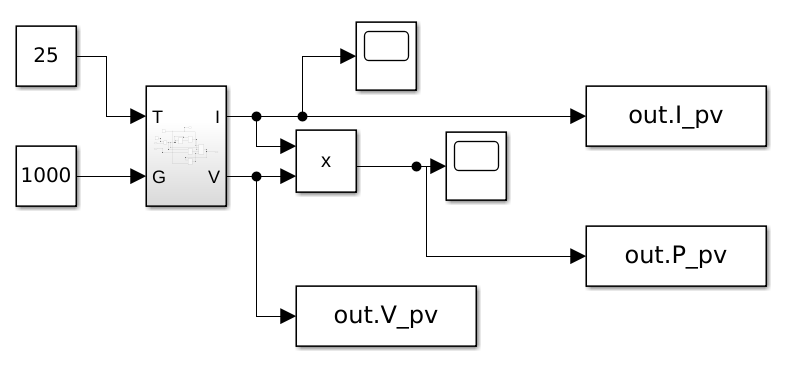
\includegraphics[width=0.9\textwidth]{./imagenes/simulink1.png}
		\caption{Arreglo PV}
	\end{figure} 
	
	Así mismo, se parte del modelo de los cinco parámetros, en donde la corriente y la tensión de salida se ven gobernadas por los siguientes ecuaciones representadas en subsistemas: 

	\begin{figure}[htb]
		\centering
		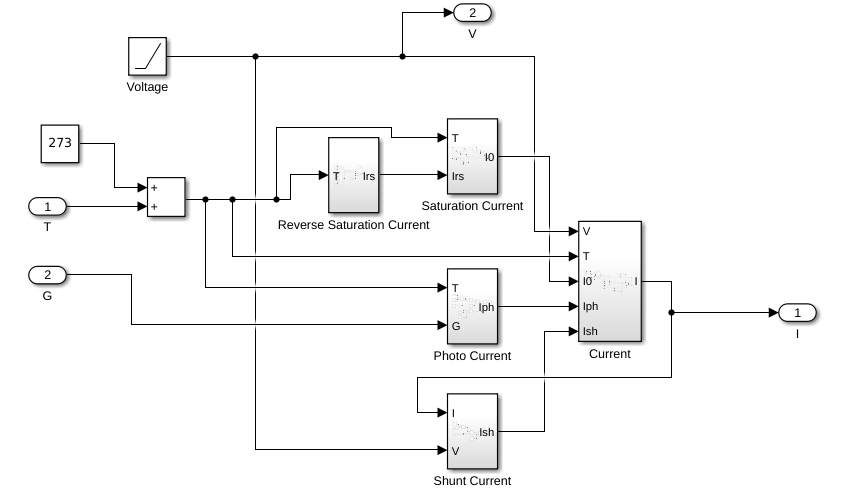
\includegraphics[width=0.9\textwidth]{./imagenes/simulink2.png}
		\caption{Sub-sistemas del modelo}
	\end{figure} 
	
	\newpage
	
	
	
	\begin{itemize}
		\item Fotocorriente
		
	
		
			\begin{equation*}
				I_{ph} = \left(I_{sc} + K_i \times \left(T - 298 \right) \right) \times \left(G/1000 \right)
			\end{equation*}
			
			\begin{figure}[h!]
				\centering
				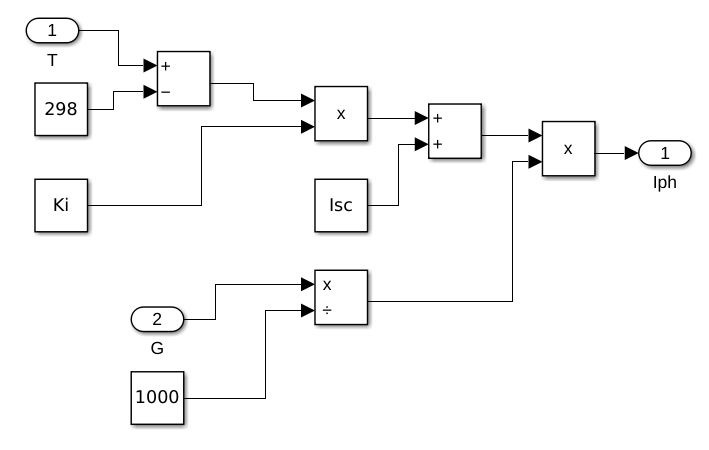
\includegraphics[width=0.75\textwidth]{./imagenes/simulink3.png}
				\caption{Subsistema para Fotocorriente}
			\end{figure} 
		
		\item Corriente de saturación
		
			\begin{equation*}
				I_o = I_{rs} \times \left( \frac{T}{T_n} \right)^3 \times \exp \left( \left( q \times E_{go} \times \left(1/T_n - 1/T \right) \right)/ \left(n \times k \right) \right)
			\end{equation*}
			
			\begin{figure}[htb]
				\centering
				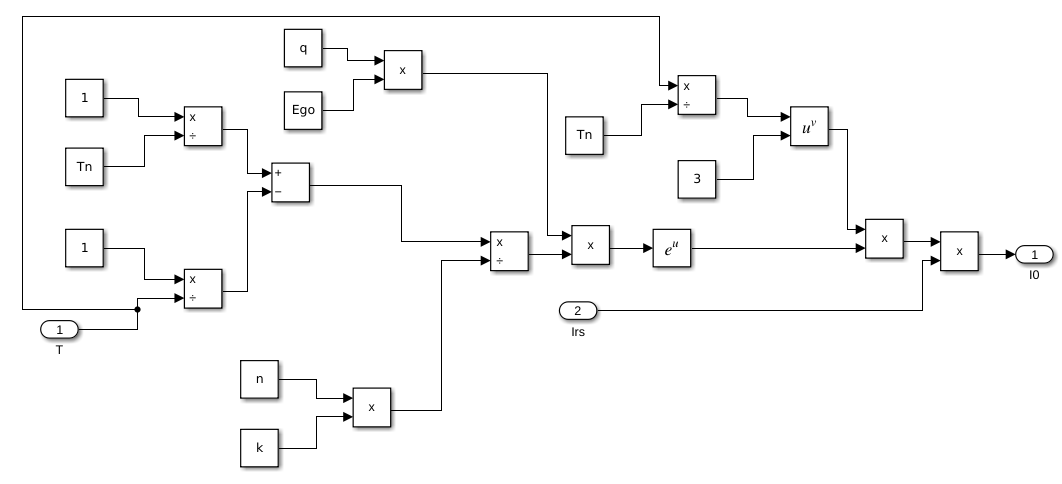
\includegraphics[width=0.9\textwidth]{./imagenes/simulink4.png}
				\caption{Subsistema de Corriente de saturación}
			\end{figure}
		
		\newpage
		
		\item Corriente de saturación reversa
		
			\begin{equation*}
				I_{rs} = I_{sc} / (\exp((q*V_{oc})/(n*N_s*k*T ))-1)
			\end{equation*}
			
			\begin{figure}[htb]
				\centering
				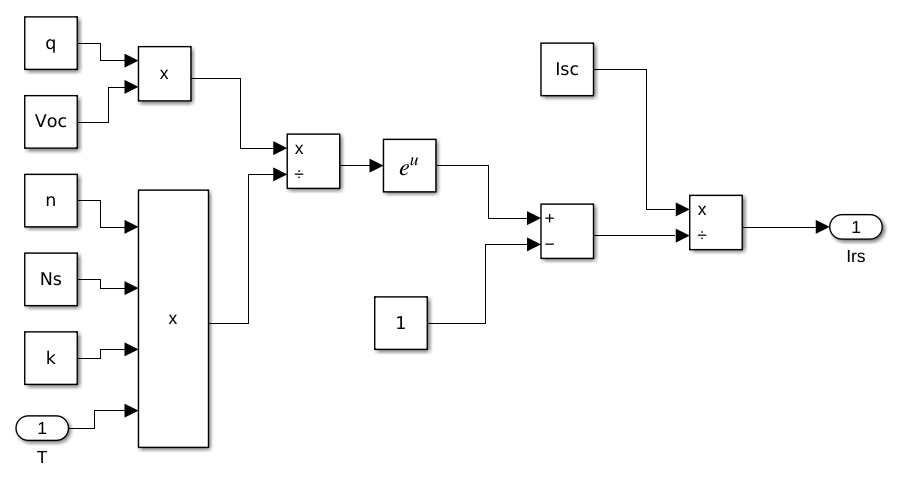
\includegraphics[width=0.9\textwidth]{./imagenes/simulink5.png}
				\caption{Subsistema de Corriente de saturación reversa}
			\end{figure}
		
		\item Corriente shunt
		
			\begin{equation*}
				I_{sh} = (V +I*R_s)/R_{sh}
			\end{equation*}
			
			\begin{figure}[htb]
				\centering
				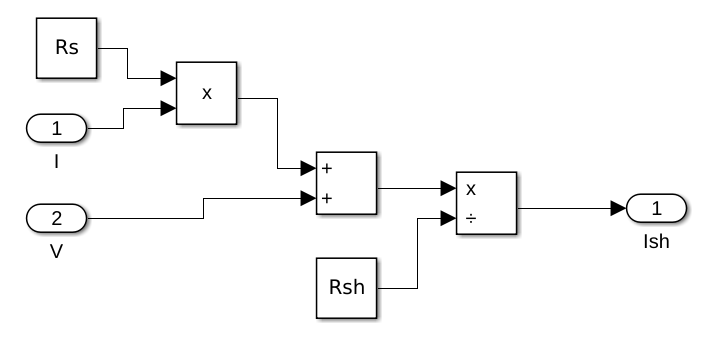
\includegraphics[width=0.9\textwidth]{./imagenes/simulink6.png}
				\caption{Subsistema de la corriente shunt}
			\end{figure} 
		
		\newpage
		
		\item Corriente de salida
		
			\begin{equation*}
				I = I_{ph}*NP - I_o * NP *(\exp((q*(V/NS + I*R_s/NP))/(n*N_s*k*T))-1)-I_{sh}
			\end{equation*}
			
			\begin{figure}[htb]
				\centering
				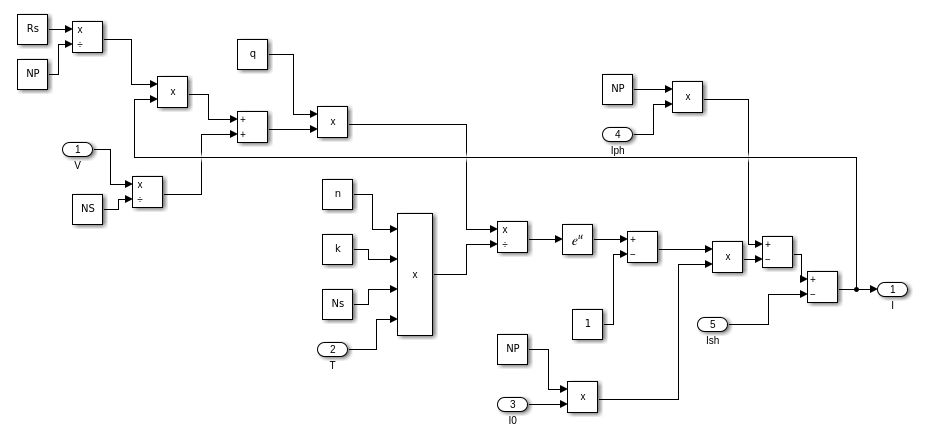
\includegraphics[width=0.9\textwidth]{./imagenes/simulink7.png}
				\caption{Subsistema de la corriente de salida}
			\end{figure} 
		
		Los resultados son almacenados en un archivo CSV para su fácil manipulación en otros lenguajes como Python.
		
		Las curvas características que se obtienen del arreglo fotovoltaico son:
		
		\lstinputlisting[language=Python, firstline=12, lastline=39]{graficas.py}
		
		\begin{figure}[htb]
			\centering
			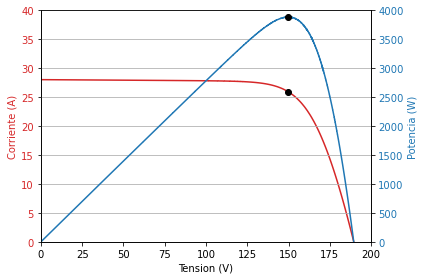
\includegraphics[width=0.8\textwidth]{./imagenes/curvacaracteristica.png}
			\caption{Curvas características}
		\end{figure} 
		

Se hace uso de la función \texttt{numpy.poly1d()} que nos ayuda a definir una función polinomial de la siguiente manera:

		\lstinputlisting[language=Python, firstline=42, lastline=64]{graficas.py}

		\begin{figure}[htb]
			\centering
			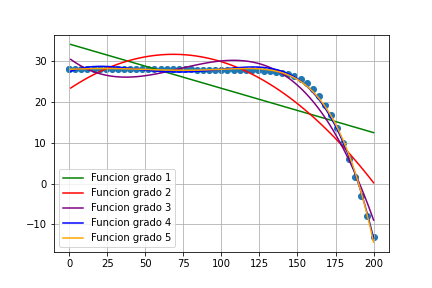
\includegraphics[width=0.9\textwidth]{./imagenes/curvaajuste.png}
			\caption{Funciones Polinomiales}
		\end{figure} 
	
Los resultados del R ajustado para cada modelo se obtienen de la siguiente función, y están organizados en la tabla:

\lstinputlisting[language=Python, firstline=67, lastline=77]{graficas.py}
		
	\end{itemize}
	
	\begin{tabular}{| c | c |}
		\hline
		Modelo & R cuadrado ajustado \\ \hline
		Grado 1 & 0.4376094058571091 \\
		Grado 2 & 0.7969866148484753 \\
		Grado 3 & 0.9606980241040581 \\
		Grado 4 & 0.9968071975795516 \\
		Grado 5 & 0.9984087544931406 \\ \hline
	\end{tabular}
	 
	
	 Se selecciona el modelo de grado 5:
	 
	 \begin{figure}[htb]
	 	\centering
	 	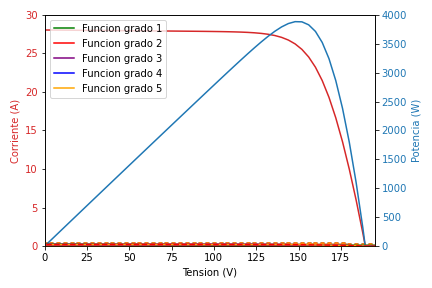
\includegraphics[width=0.9\textwidth]{./imagenes/modeloSel.png}
	 	\caption{Modelo seleccionado}
	 \end{figure}
	 
	El resultado de los coeficientes de la función polinómica de grado 5 es:
	
	\begin{equation*}
		i(v) = -8.713\times 10^{-10}v^5 + 2.213\times 10^{-7} v^4 - 1.538\times 10^{-5} v^3 + 7.92\times 10^{-5} v^2 + 0.01166 v + 27.93
	\end{equation*}

\end{document}